\documentclass{beamer}
\usepackage{beamerthemesplit}
\usepackage{color}
\usepackage{amsfonts}
\usepackage{multimedia}
\usepackage{animate}
\usepackage{wrapfig}
\usepackage{multicol}
%\setlength{\textwidth}{15cm}           %Sets the width of the printable area of the page to 15cm
%\setlength{\topmargin}{0cm}            %Space from the toprule to the top of the text (first line) to 0 cm.
%\setlength{\footskip}{0cm}               %Space from the bottom of the text to the footnote (or footrule) to 0 cm.
\setlength{\marginparwidth}{0cm}   
\setlength{\columnsep}{0cm}


\definecolor{cvggreen}{RGB}{4,71,79}
\mode<presentation>
{
%Darmstadt
\usetheme[]{Amsterdam}
}
\title{Marchiatura digitale di sequenze video stereoscopiche a disparit\`{a} coerente}
\author{Benedetta Barbetti\\ 
		Michaela Servi}
\institute{Universit\`{a} degli studi di Firenze}
\date{10 Dicembre 2015}


\begin{document}

\begin{frame}
\titlepage
\end{frame}

\begin{section}{Introduzione}
\subsection{Video Stereoscopici}

\begin{frame}[t]{\textsc{Contesto}}
Numerose applicazioni di elaborazione di immagini e video richiedono esplicite informazioni sulla \textbf{profondit\`{a}} della scena:
\setlength{\columnsep}{0cm}
\begin{columns}
\begin{column}{4cm}
\begin{center}
\setbeamertemplate{blocks}[rounded][shadow=false]
	\setbeamercolor{block body}{use=structure,fg=black,bg=lightgray} 	
\begin{block}{Campi applicativi}
		\begin{itemize}
			\item \small{Medicina} 
			\item Robotica
			\item Tracking
			\item Industria manifatturiera
			\item Cinema
		\end{itemize}	
	\end{block}
	
%	\textbf{Caratteristiche}:
%			\vspace*{0.5em}
%			%\begin{small}
%			\begin{itemize}
%			\item \small{Medicina} 
%			\item Robotica
%			\item Tracking
%			\item Industria manifetturiera
%			\item Cinema
%			\end{itemize}
%			%\end{small}

\end{center}
\end{column}
\begin{column}{6cm}
\begin{figure}
\centering
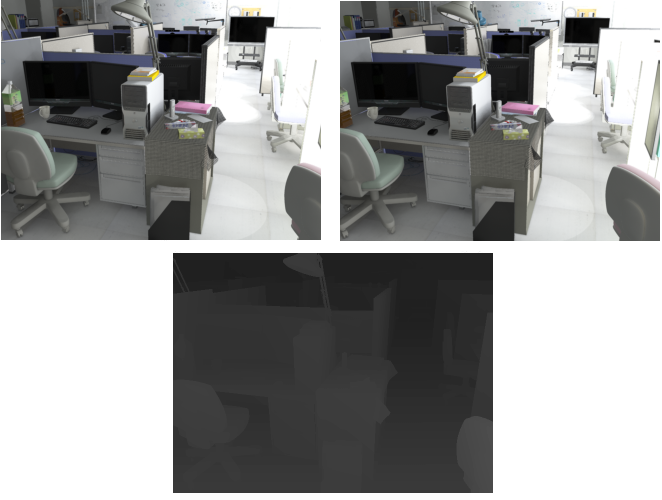
\includegraphics[width=1\linewidth]{./img/track.png}
\end{figure}
\end{column}
\end{columns}
\end{frame}


\begin{frame}[t]{\textsc{Video Stereoscopici}}
	\setbeamertemplate{blocks}[rounded][shadow=false]
	\setbeamercolor{block title}{use=structure,fg=black,bg=lightgray} 
	\setbeamercolor{block body}{use=structure,fg=black,bg=lightgray} 	
\begin{block}
	\center{Il \textbf{video stereoscopico} \`{e} ottenuto da due riprese con una \textbf{coppia di telecamere} adiacenti successivamente sovrapposte}
\end{block}
	\vspace{1em}
\begin{center}
\movie[width=8cm,height=5cm,autostart,loop,poster]{}{./img/alice.mp4}
\end{center}
\end{frame}





\begin{frame}[t]{\textsc{Dispositivi di ripresa e visualizzazione}}
\begin{columns}
\begin{column}{5cm}
\begin{center}
\setbeamertemplate{blocks}[rounded][shadow=false]
	\setbeamercolor{block body}{use=structure,fg=black,bg=lightgray} 
	\setbeamerfont{block body}{size=\tiny}	
\begin{block}{Sistema di ripresa stereo}
		\begin{itemize}
			\item  \small{Due telecamere sincronizzate}
			\item \small{Correttamente allineate}
			\item \small{Stessa calibrazione}
		\end{itemize}	
	\end{block}
\end{center}
\centering
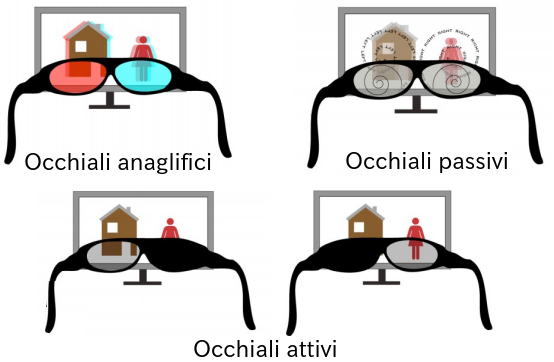
\includegraphics[width=1\linewidth]{./img/display.png}
\end{column}

\begin{column}{5cm}

\centering
\vspace{0.7em}
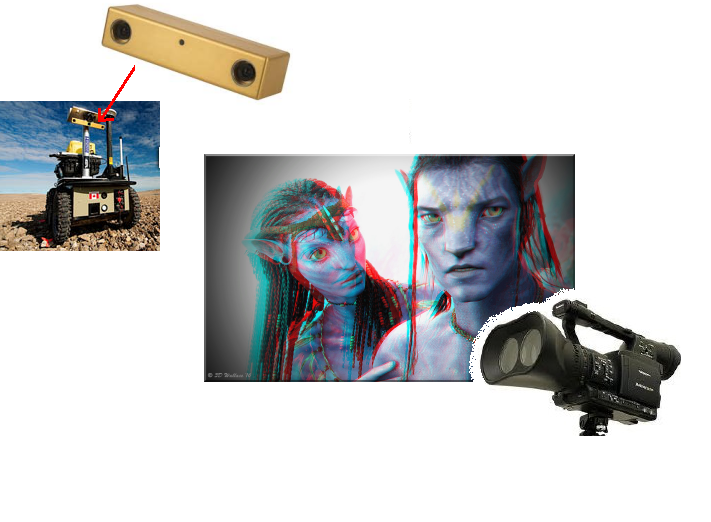
\includegraphics[width=1\linewidth]{./img/camere.png}
\vspace{-2.8em}
\begin{center}
\setbeamertemplate{blocks}[rounded][shadow=false]
	\setbeamercolor{block body}{use=structure,fg=black,bg=lightgray} 		
\begin{block}{Sistema di riproduzione}
		\begin{itemize}
			\item  \small{Attivo: lenti sincronizzate con il televisore}
			\item \small{Passivo: lenti diversamente polarizzate}
			\item \small{Anaglifico: lenti passive con filtri di colore diverso}
		\end{itemize}	
	\end{block}
\end{center}
\end{column}
\end{columns}
\end{frame}








\begin{frame}[t]{\textsc{Necessit\`{a} di una marchiatura}}
	\setbeamertemplate{blocks}[rounded][shadow=false]

	\setbeamercolor{block body}{use=structure,fg=black,bg=lightgray} 	
\begin{center}
\begin{block}{Precedenti motivazioni}
\begin{itemize}
\item  Sicurezza
\item  Copyright
\end{itemize}
\end{block}
\vspace{2em}
\begin{block}{Nuove motivazioni}
\begin{itemize}
\item Migliorare la qualit\`{a} visiva dei contenuti marchiati utilizzando la particolarit\`{a} dei contenuti
\end{itemize}
\end{block}
\end{center}
\end{frame}


\begin{frame}[t]{\textsc{Scopo di questa tesi}}


\end{frame}

\end{section}

\begin{section}{Stereoscopia}
\subsection{Principi della stereoscopia}
\begin{frame}[t]{\textsc{Stereoscopia}}

\end{frame}

\end{section}


\begin{section}{Watermarking}
\subsection {Principi del watermarking}
\begin{frame}[t]{\textsc{Watermarking}}

\end{frame}


\end{section}
\begin{section}{Stato dell'Arte}
\subsection{Watermarking di video stereoscopici}
\begin{frame}[t]{\textsc{Stato dell'arte}}

\end{frame}

\begin{frame}[t]{\textsc{Metodi a Disparit\`{a} Coerente}}
\end{frame}

\end{section}

\begin{section}{Metodo implementato}
\begin{frame}[t]{\textsc{Marchiatura digitale spaziale a disparit\`{a} coerente}}

\end{frame}
\end{section}




\end{document}
